\noindent

\includegraphics[height=1.25cm]{images/pictograms/triangle}

\includegraphics[height=1.25cm]{images/pictograms/tools}

%%%%%%%%%%%%%%%%%%%%%%%%%%%%%%%%%%%%%%%%%%%%%%%%%%%%%%%%%%%%%%%%%%%%%%%%%%%%%%%%%%%%%%%%%%%%%%%%%%%

\begin{flushright} {\tiny {\color{gray} python\_codes/fieldstone\_172/text.tex}} \end{flushright}

%\lstinputlisting[language=bash,basicstyle=\small]{python_codes/template_keywords.key}

\par\noindent\rule{\textwidth}{0.4pt}

\begin{center}
\inpython
{\small Code: \url{https://github.com/cedrict/fieldstone/tree/master/python_codes/fieldstone_172}}
\end{center}

\par\noindent\rule{\textwidth}{0.4pt}

Last revision: March 24th, 2025.

\par\noindent\rule{\textwidth}{0.4pt}

%%%%%%%%%%%%%%%%%%%%%%%%%%%%%%%%%%%%%%%%%%%%%%%%%%%%%%%%%%%%%%%%%%%%%%%%%%%%%%%%%%%%%%%%%%%%%%%%%%%


At \url{https://en.wikipedia.org/wiki/Sierpinski_triangle} we 
read
\begin{displayquote}
{\color{darkgray}
The Sierpiński triangle, also called the Sierpiński gasket or Sierpiński sieve, is a fractal 
with the overall shape of an equilateral triangle, subdivided recursively into smaller 
equilateral triangles. Originally constructed as a curve, this is one of the basic 
examples of self-similar sets--that is, it is a mathematically generated pattern 
reproducible at any magnification or reduction. It is named after the Polish 
mathematician Wacław Sierpiński but appeared as a decorative pattern many centuries before 
the work of Sierpiński. 

[...]

Start by labeling $\vec{p}_0$, $\vec{p}_1$ and $\vec{p}_2$ 
as the corners of the Sierpiński triangle, 
and a random point $\vec{r}_0$. 
Set $\vec{r}_{n+1} = \frac12 (\vec{r}_n+\vec{p}_{r_n})$, 
where $r_n$ is a random number 0, 1 or 2. 
Draw the points $\vec{r}_0$ to $\vec{r}_\infty$. 
}
\end{displayquote}

More simply, the algorithm is as follows:

\begin{enumerate}
\item Take three points in a plane to form a triangle.
\item Randomly select any point inside the triangle and consider that your current position.
\item Randomly select any one of the three vertex points.
\item Move half the distance from your current position to the selected vertex.
\item Plot the current position.
\item Repeat from step 3.
\end{enumerate}

%%%%%%%%%%%%%%%%%%%%%%%%%%%%%%5
\section*{Implementation}

The code is actually very simple.
We first choose three vertices:
\begin{lstlisting}
x=[1.,3.,2.]
y=[1.,1.5,2.5]
\end{lstlisting}
and then select a starting point chosen at random inside the 
triangle:

\begin{lstlisting}
r=random.uniform(0,1)
s=random.uniform(0,1-r)
N[0]=1-r-s
N[1]=r
N[2]=s
xpt=N.dot(x)
ypt=N.dot(y)
\end{lstlisting}
where we have used the 1st-order $P_1$ basis functions to compute the 
coordinates of the point after its reduced coordinates $r,s$ were
randomly generated inside the reference triangle.

Having chosen the number of points \lstinline{npts} to be generated inside the 
triangle we apply the algorithm highlighted above:

\begin{lstlisting}
for k in range(0,npts):
    ivertex=random.randint(0,2)
    xcoords[k]=(xpt+x[ivertex])/2
    ycoords[k]=(ypt+y[ivertex])/2
    xpt=xcoords[k]
    ypt=ycoords[k]
\end{lstlisting}

The code implements a loop on \lstinline{npts} and exports the 
resulting generated points to an ascii file later to be plotted with gnuplot. 

%%%%%%%%%%%%%%%%%%%%%%%%%%%%%%%%%%%%%%%%
\section*{Results}

\begin{center}
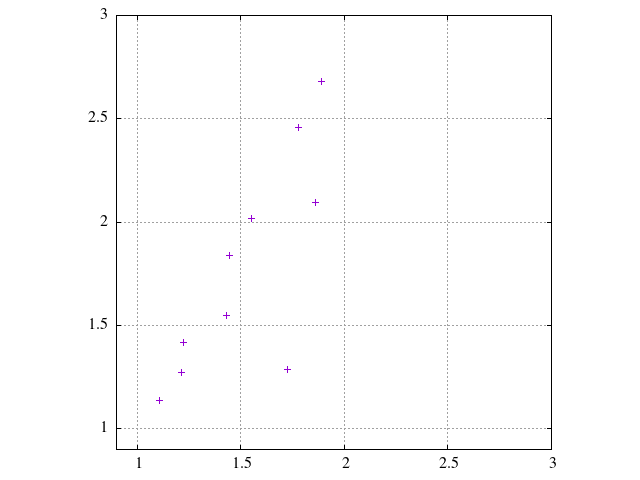
\includegraphics[width=5.7cm]{python_codes/fieldstone_172/results/pts_10.png}
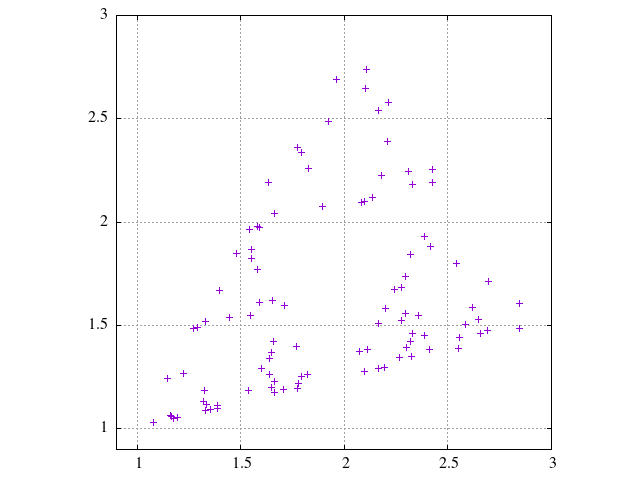
\includegraphics[width=5.7cm]{python_codes/fieldstone_172/results/pts_100.png}
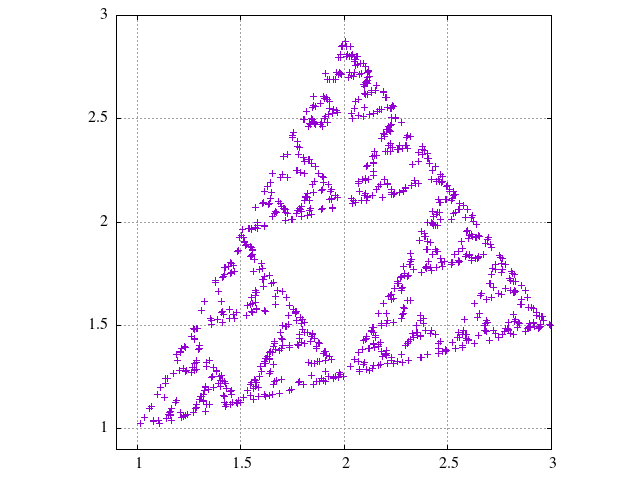
\includegraphics[width=5.7cm]{python_codes/fieldstone_172/results/pts_1000.png}\\
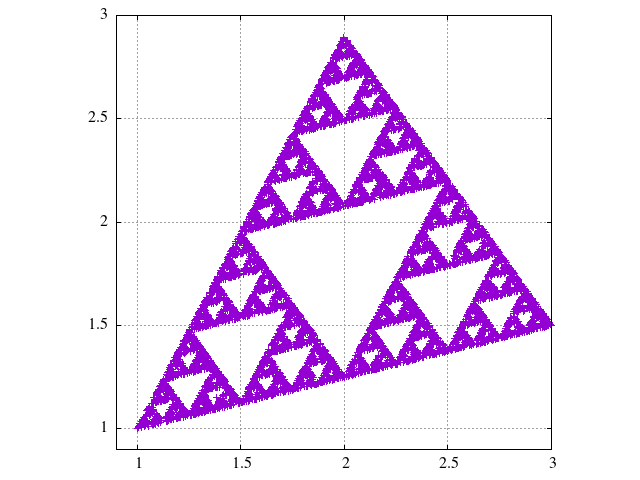
\includegraphics[width=8cm]{python_codes/fieldstone_172/results/pts_10000.png}
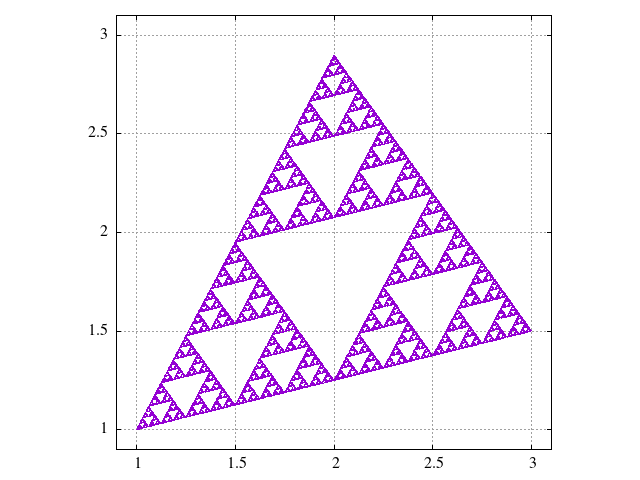
\includegraphics[width=8cm]{python_codes/fieldstone_172/results/pts_100000.png}\\
{\captionfont Results obtained for npts=10,100,1000,10000,100000.}
\end{center}


Note the interesting video by Numberphile about this topic: \url{https://www.youtube.com/watch?v=FnRhnZbDprE}













